\documentclass[border=6pt]{standalone}
% Shared preamble for web figures.  Each figure is a standalone .tex that
% \input's this file; scripts/make-figures.sh turns it into an SVG.
% Handouts pull the same file with \fig{Unit_X/<name>}.
\usepackage[T1]{fontenc}
\usepackage{helvet}
\renewcommand{\familydefault}{\sfdefault}
\usepackage{amsmath}
\usepackage{tikz}
\usetikzlibrary{arrows.meta,positioning,calc,shapes.symbols,shapes.geometric}

% Who makes the rules is the point of most diagrams in this book, so the
% colors mean the same thing everywhere: blue is a person, orange is the
% computer, green is an answer, pink is the human brain.
\definecolor{person}{HTML}{2C6FAE}
\definecolor{machine}{HTML}{D35400}
\definecolor{result}{HTML}{1E8449}
\definecolor{brainpink}{HTML}{C2185B}
\definecolor{ink}{HTML}{2C3E50}

\tikzset{
  doodle/.style={line width=1.5pt, line cap=round, line join=round, draw=ink},
  box/.style={draw, rounded corners=5pt, line width=1.1pt, align=center,
              inner sep=7pt, minimum height=1.0cm, font=\small},
  personbox/.style={box, draw=person, fill=person!10},
  machinebox/.style={box, draw=machine, fill=machine!10},
  resultbox/.style={box, draw=result, fill=result!10},
  plainbox/.style={box, draw=ink!70, fill=ink!4},
  flow/.style={-{Stealth[length=8pt]}, line width=1.4pt, draw=ink},
}

\begin{document}
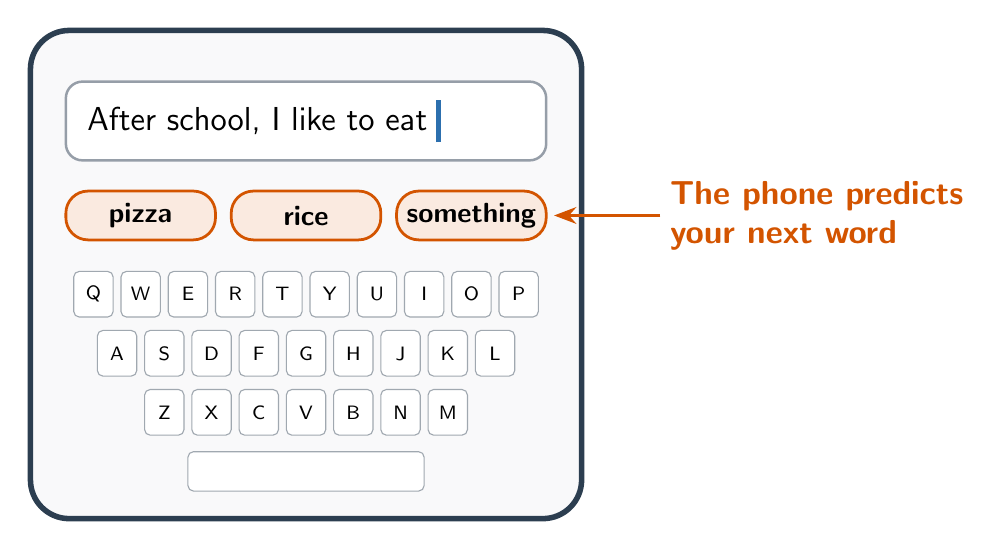
\begin{tikzpicture}
% A phone keyboard suggesting the next word.
\draw[ink, line width=2pt, rounded corners=14pt, fill=ink!3] (0,0) rectangle (7,6.2);
\draw[ink!50, rounded corners=6pt, fill=white, line width=0.9pt] (0.45,4.55) rectangle (6.55,5.55);
\node[anchor=west, font=\large] (t) at (0.6,5.05) {After school, I like to eat};
\draw[person, line width=1.6pt] ($(t.east)+(0.02,-0.27)$) -- ($(t.east)+(0.02,0.27)$);

% suggestion bar
\foreach \x/\w in {1.4/pizza, 3.5/rice, 5.6/something} {
  \node[draw=machine, fill=machine!12, rounded corners=8pt, line width=1pt,
        minimum width=1.9cm, minimum height=0.62cm, font=\bfseries] at (\x,3.85) {\w};
}

% keys
\foreach \k [count=\i from 0] in {Q,W,E,R,T,Y,U,I,O,P}
  \node[draw=ink!45, fill=white, rounded corners=2pt, minimum width=0.5cm, minimum height=0.58cm,
        inner sep=0pt, font=\scriptsize] at (0.8+0.6*\i,2.85) {\k};
\foreach \k [count=\i from 0] in {A,S,D,F,G,H,J,K,L}
  \node[draw=ink!45, fill=white, rounded corners=2pt, minimum width=0.5cm, minimum height=0.58cm,
        inner sep=0pt, font=\scriptsize] at (1.1+0.6*\i,2.1) {\k};
\foreach \k [count=\i from 0] in {Z,X,C,V,B,N,M}
  \node[draw=ink!45, fill=white, rounded corners=2pt, minimum width=0.5cm, minimum height=0.58cm,
        inner sep=0pt, font=\scriptsize] at (1.7+0.6*\i,1.35) {\k};
\draw[ink!45, fill=white, rounded corners=2pt] (2.0,0.35) rectangle (5.0,0.85);

% label
\node[align=left, anchor=west, font=\large\bfseries, text=machine] (lab) at (8.0,3.85)
  {The phone predicts\\your next word};
\draw[flow, draw=machine] (lab.west) -- (6.65,3.85);
\end{tikzpicture}
\end{document}
